\chapter{Polarization and Interference}
\section{Introduction}
You have already investigated some wave properties last semester, so here we will expand upon your knowledge of waves and address three new concepts: polarization, interference and diffraction. Our experiment will be conducted with light waves, however the general concepts apply to many other waves as well.

\section{Theory}
\subsection{Polarization}
Polarization occurs only in transverse waves\footnote{Examples of transverse waves are oscillations on a string, water waves, or the electromagnetic radiation we treat here. Sometimes you may also hear the term polarization used in the context of transverse- and longitudinal polarization.}. By definition, the oscillation is perpendicular to the direction of wave propagation in a transverse wave. Since in three-dimensional space there are three independent dimensions, there are two possible perpendicular directions needed to describe any oscillatory motion perpendicular to the direction of motion. If you think about a transverse wave in a string, the oscillation could be up-and-down or left-and-right, while the wave front propagates forward along the string. The two independent and perpendicular directions are called the two polarization states. (Or in coordinates, if a wave propagates along the $z$-axis, there are two polarizations perpendicular to the wave motion--one along the $x$-axis and one along the $y$-axis.) Polarization cannot occur in longitudinal waves because the direction of oscillation has only one possibility, along the direction of motion.\myskip

You may argue that you can make oscillations happen on a string in more than just the two directions described above--and you are right! For example, you can make oscillations diagonally from the upper left to the lower right or you can even make circular oscillations by moving your hand continuously in a circle, producing a corkscrew pattern along the string\footnote{This wave is sometimes called left- or right- circular polarization.}. But no matter which wave you make, the oscillations can always be represented as two superimposed waves with displacements along the two mutually perpendicular polarization axes. Any vector can always be described by decomposing it into its $x$- and $y$- components. Here, the relevant vector is the oscillating displacement from the $z$-axis. The amplitudes of the resolved $x$ and $y$ components indicate how much of the wave is in each polarization state.\myskip

For electromagnetic radiation, the oscillating quantities are the electric (and magnetic) fields. These undulate perpendicular to the direction of the wave. Like waves in a string, electromagnetic waves are transverse waves and have polarization properties. The polarization state describes the axis along which the electric field in the wave oscillates. Visible light is electromagnetic radiation in a particular frequency-wavelength regime, with large frequency of oscillation ($\sim 10^{15}\,\mathrm{Hz}$) and small wavelength ($\sim 0.5\times 10^{-6}\, \mathrm{m}$).\myskip

\subsection{Polarizer}
Usually light is produced (e.g. incandescent light from a candle or a light bulb) by hot electrons and atoms, which are moving or are oriented in random directions, so that the wave is \textbf{unpolarized}. This means that the electric field associated with the wave oscillates in random directions (though always at right angles to the direction of the propagation of the light). So there is no favored direction for polarization. It is as if you were moving your hand in random directions at the end of a string. Note that this is very different from the cases of waves in a string described above. Even in circular polarization the oscillations were not random.
\begin{figure}[h]
\centering
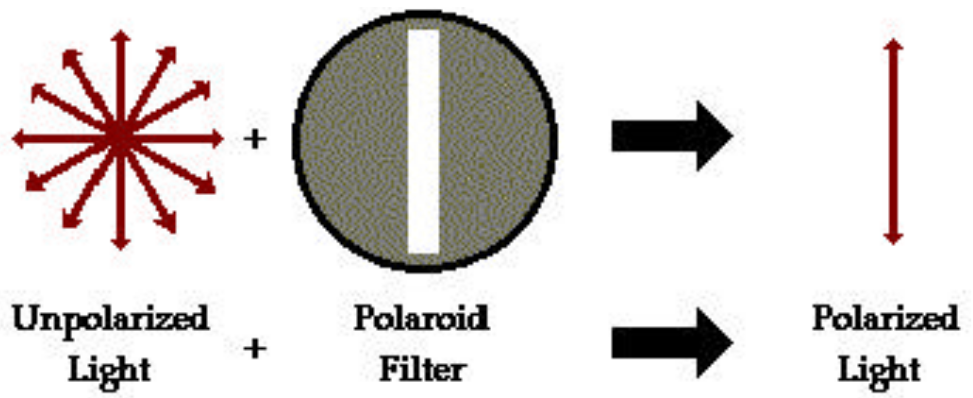
\includegraphics[width=0.5\textwidth]{./Exp8/pic/image1.png}
\caption{Polarization Filter and Creation of Polarized Light}
\label{fig:creation}
\end{figure}

A polarization filter, shown in Figure {\ref{fig:creation}}, is a device with a specified direction, called the polarization axis. The filter absorbs all the wave's incoming electric field perpendicular to the polarization axis and transmits the electric field parallel to the polarization axis. So no matter what the polarization of the light shining into a polarizer might be, the light coming out of the polarizer is always polarized in the direction specified by the polarization axis\footnote{Such light is called linearly polarized light.}. An unpolarized wave just prior to the polarizer has an electric field ($\mathbf{E}$) pointing randomly in all directions perpendicular to the wave direction, as shown in Figure {\ref{fig:detection}}. The polarized wave after the polarizer has only half the energy content, and the $\mathbf{E}$-field is oscillating solely along the polarization axis. This electric field has the same value as the component along that axis just before the polarizer.
\begin{figure}[h]
\centering
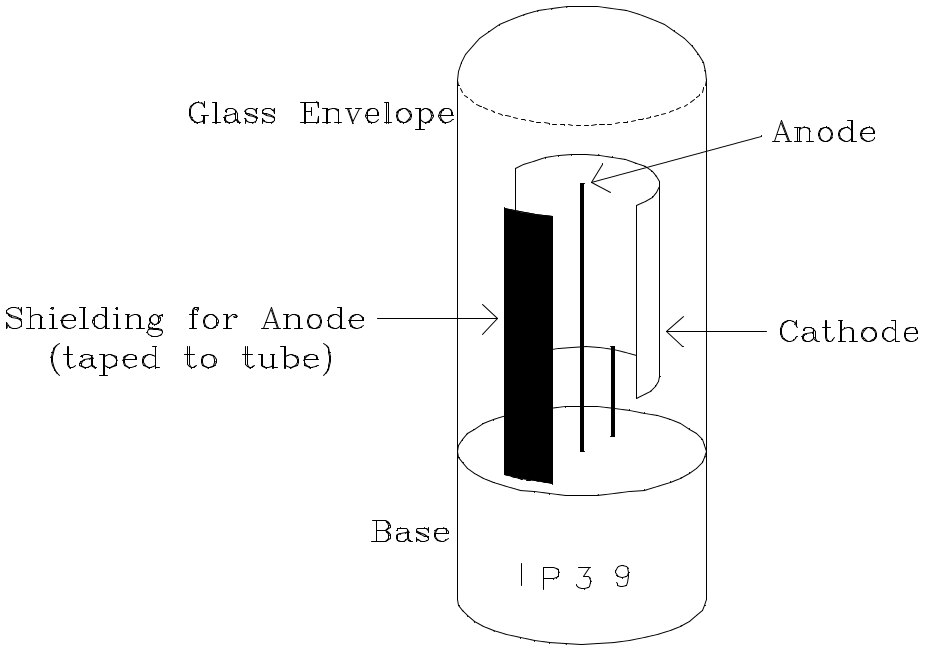
\includegraphics[width=0.8\textwidth]{./Exp8/pic/image2.png}
\caption{Detection of Polarized Light}
\label{fig:detection}
\end{figure}

\subsection{Interference--The Double Slit}
As you've learned in class, Young's double slit experiment is a demonstration of interference and diffraction. A double slit, as illustrated in Figure {\ref{fig:double}}, permits what remains of an incoming wave (from the left) to travel to a distant screen (to the right) along two different paths with different lengths. The light waves from the two slits interfere, resulting in an interference pattern of bright (constructive) and dim (destructive) patches as viewed on the screen. Let's see how the double slit works using Figure {\ref{fig:double}}.
\begin{figure}[h]
\centering
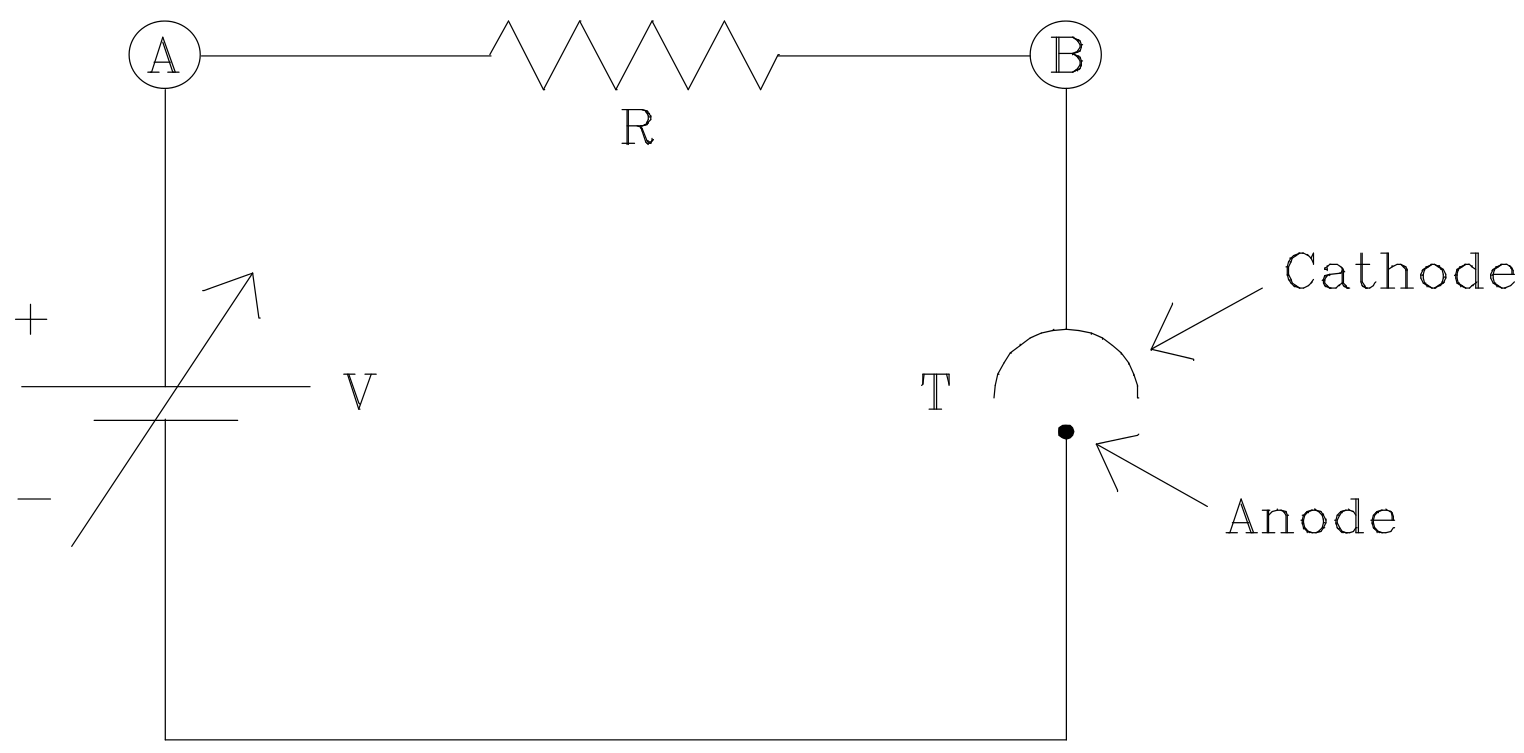
\includegraphics[width=0.8\textwidth]{./Exp8/pic/image3.png}
\caption{Young's Double Slit Experiment}
\label{fig:double}
\end{figure}

We shine light from the left onto the double slit, which allows two light waves to propagate from the two slits. Straight-ahead they will always be in phase since they travel the same distance to the screen. But when the two waves propagate at an angle $\theta$, they cover different distances to reach a specific point on the screen. (We assume that the two rays are parallel, a good approximation since the screen is effectively infinitely far away compared to the distance between the two slits.)\myskip
\begin{figure}[h]
\centering
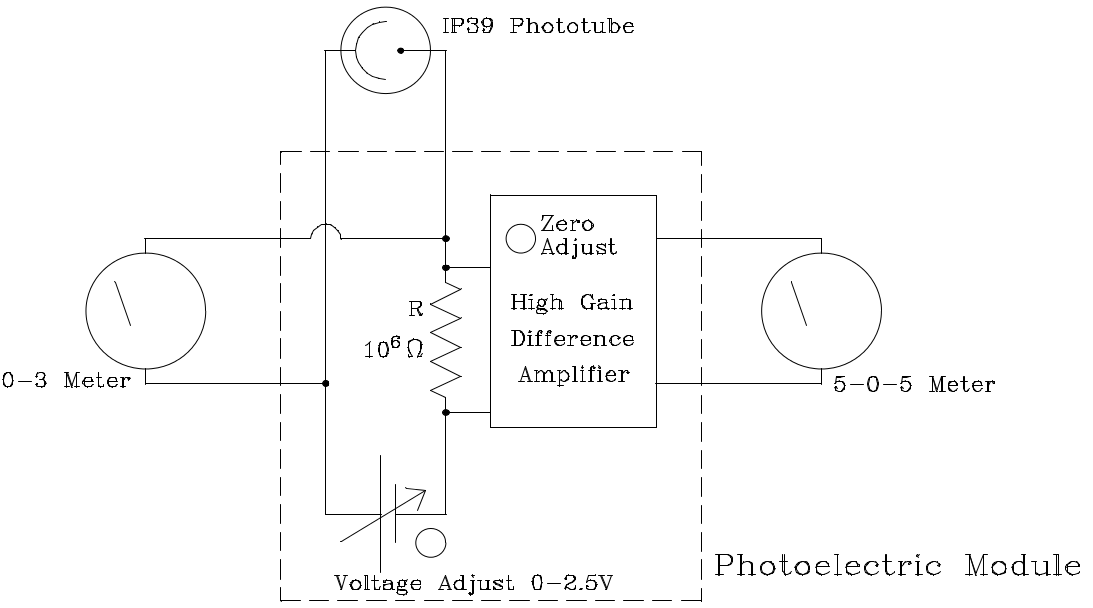
\includegraphics[width=0.3\textwidth]{./Exp8/pic/image4.png}
\caption{Geometry of the Double Slit}
\label{fig:geometry}
\end{figure}

As you can convince yourself by applying the rules of trigonometry to the triangle in Figure {\ref{fig:geometry}}, the difference in path ($\Delta l$) between the two rays is, for slit separation, $d$,
\begin{equation}
 \Delta l =d\sin\theta
\end{equation}

So what quantitatively determines a point of maximum intensity on the screen? Maximum intensity occurs if the two waves are precisely in phase at that point on the screen. This follows from what you learned about constructive and destructive interference in the lab on standing waves. As you saw, two waves can add up constructively or destructively. In the case of maximal constructive interference, the waves combine at the screen so that a crest on one wave coincides with a crest on the other wave and a trough coincides with a trough. In the case of maximal destructive interference, the waves combine so that a crest on one wave coincides with a trough on the other wave. \myskip

The waves will be in phase when they meet at the screen if the path difference between the two waves is an exact number of wavelengths, $m$, where $m$ is an integer called the order of the maximum. This requirement, expressed mathematically, is
\begin{equation}
 \Delta l =m\lambda
\end{equation}

Note that if $m=0$, there is no difference in the path lengths, resulting in a maximum straight ahead, $\theta=0$, as shown in Figure {\ref{fig:interference}}. Subsequent maxima occur for subsequent positive and negative integers, $m=\pm 1, \pm 2, \pm 3, \dots$. \myskip

Combining the two equations for $\Delta l$, we get for the specific angles, $\theta_{m}$ , that give maximal constructive interference:
\begin{equation}
 d\sin \theta_{m}=m\lambda
\end{equation}

If we know the order $m$ of a particular maximum, we can determine the wavelength of the light incident on the double slit by measuring the angle of the maximum on the screen. Conversely, we can determine the order of a particular maximum, $m$, from the wavelength of the light and the angle.
\begin{figure}[h]
\centering
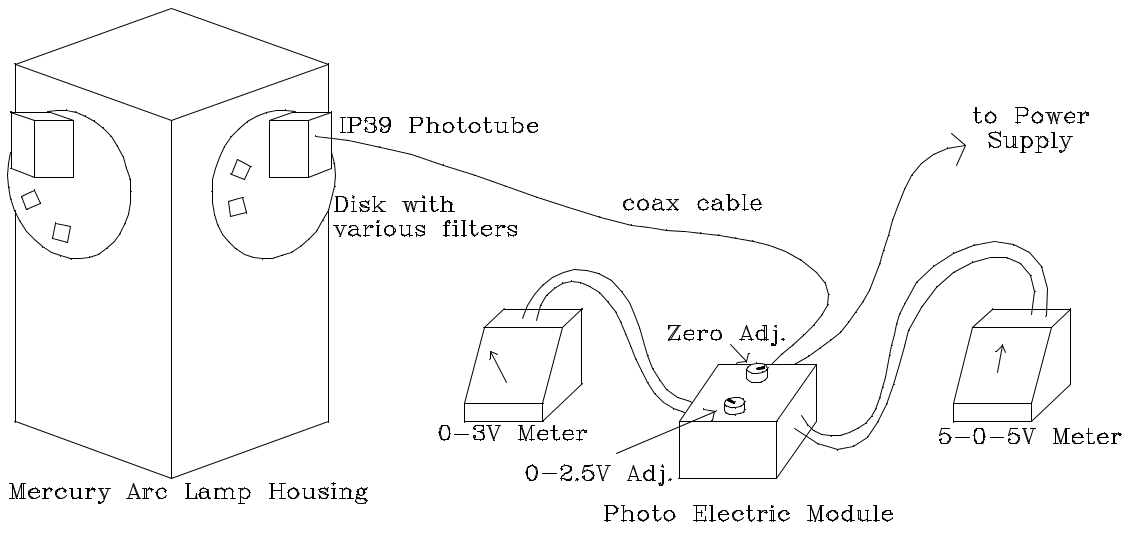
\includegraphics[width=0.6\textwidth]{./Exp8/pic/image5.png}
\caption{Interference of Light Coming from Two Small Slits}
\label{fig:interference}
\end{figure}

\subsection{Intensity of the Double-Slit Maxima}
You will soon note that the intensities for subsequent maxima are different. What causes this? Just as the double slit creates an interference pattern, each single slit creates a diffraction pattern due to interference from waves coming from different parts of a single slit as described in section 39-6 of the lecture course text\footnote{Sears, Zemansky, and Young, \textbf{College Physics \engordnumber{7} edition}, Addison-Wesley, p. 903-906.}. This occurs because each individual slit has a finite width. The overall (more realistic) pattern shown in Figure {\ref{fig:intensity}} is a superposition of the single slit and double slit interference patterns. The narrow spikes (of interest for this experiment) are due to the double slit interference and the envelope, or large-scale pattern, is due to the single slit diffraction caused by each slit.
\begin{figure}[h]
\centering
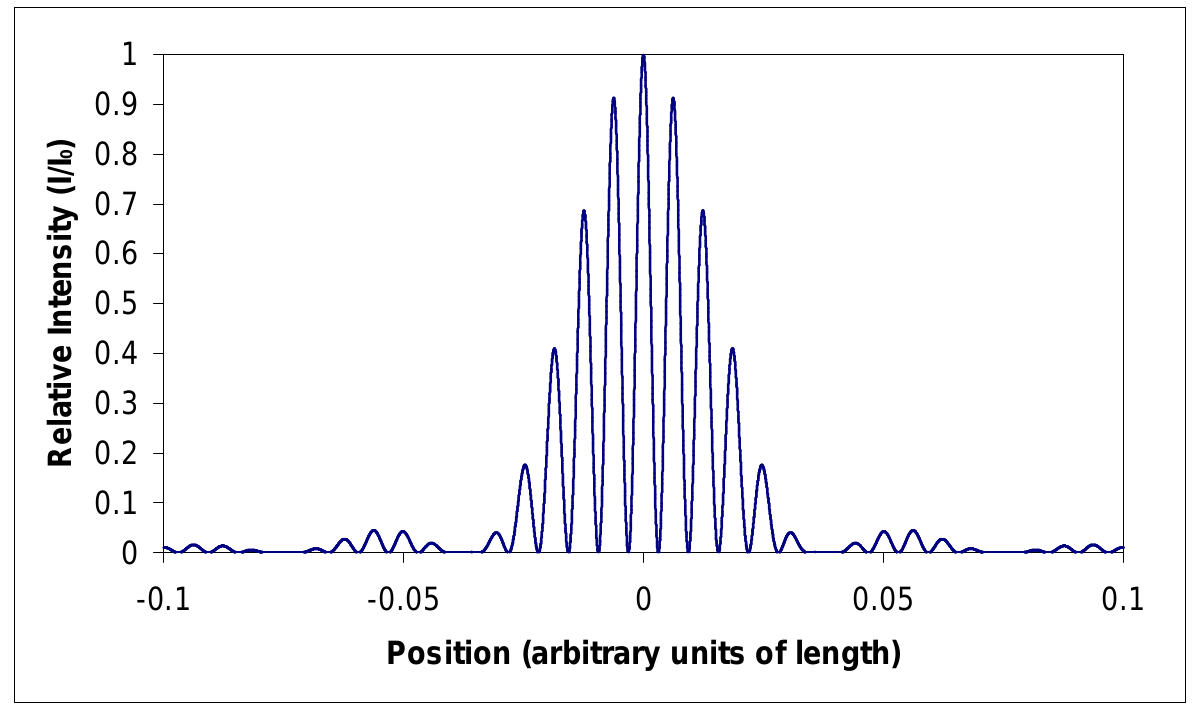
\includegraphics[width=0.8\textwidth]{./Exp8/pic/image6.png}
\caption{Intensity Pattern of the Double Slit. The Many Peaks of the Narrow Spikes Correspond to the Maxima in $d\sin\theta_{m}=m\lambda$}
\label{fig:intensity}
\end{figure}

\subsection{Light from a Laser}
In the double slit experiment we use a laser as the light source. Laser light differs from incandescent or fluorescent light in two important ways. First, lasers emit intense light of a single wavelength or frequency (monochromatic). Second, laser light is coherent, meaning that all light waves are in phase.\myskip

Let's illustrate the differences between coherent and incoherent light through a simple familiar example. Contrast a crowd of people cramming the city streets during rush hour with that of a marching band at a parade. In the midtown crowd, even if everybody were to step at the same frequency (which they don't!), each pedestrian's steps are independent of what others are doing. But the marchers at a parade move in step, or in phase, with a similar frequency, taking their steps at exactly the same time. Laser light is like the (coherent) marching band at a parade, whereas light from a light bulb is like the (incoherent) pedestrian crowd at Times Square.\myskip

Although incandescent light sources\footnote{This is easily visible in the colors produced by soap bubbles.} can produce diffraction and interference patterns, a laser is better suited to illustrate coherent phenomena.

\section{Experiment}
\subsection{Polarization}
Suppose a wave has linearly polarized light characterized by an electric field vector, $\mathbf{E}_{0}$, at an angle, $\phi$ , relative to the direction of a polarizer. The electric field that is transmitted through the polarizer is $\mathbf{E}=\mathbf{E}_{0}\cos\phi$, the component that was not absorbed. Since the energy intensity in the wave is proportional to $\mathbf{E}^2$, then the intensity passing through two polarizers will be proportional to the square of the cosine of the angle φ between the two polarizing axes.\footnote{This relation is sometimes referred to as Malus' Law, after Etienne Malus, who also discovered the polarization of reflected light in the early nineteenth century.}
\begin{equation}
 I=I_{\mathrm{max}}\cos^2\phi
\label{eq:i}
\end{equation}

In this experiment, we use an incandescent unpolarized light source and then polarize it by first passing it through a polarizer. The electric field vector $\mathbf{E}_{0}$ will then point along the same direction as the polarizing axis of the first polarizer. As the now polarized light falls on the second polarizer, only the component of $\mathbf{E}_{0}$ along the polarizing axis of the second polarizer will make it through unaffected. \myskip

As Figure {\ref{fig:polarized}} illustrates, an electric field strength of only $\mathbf{E}_{0}\cos\phi$ will make it through the second polarizer, so that the new intensity will be given by Equation {\ref{eq:i}} above. A human eye or a photometer can detect this change in light intensity.
\begin{figure}[h]
\centering
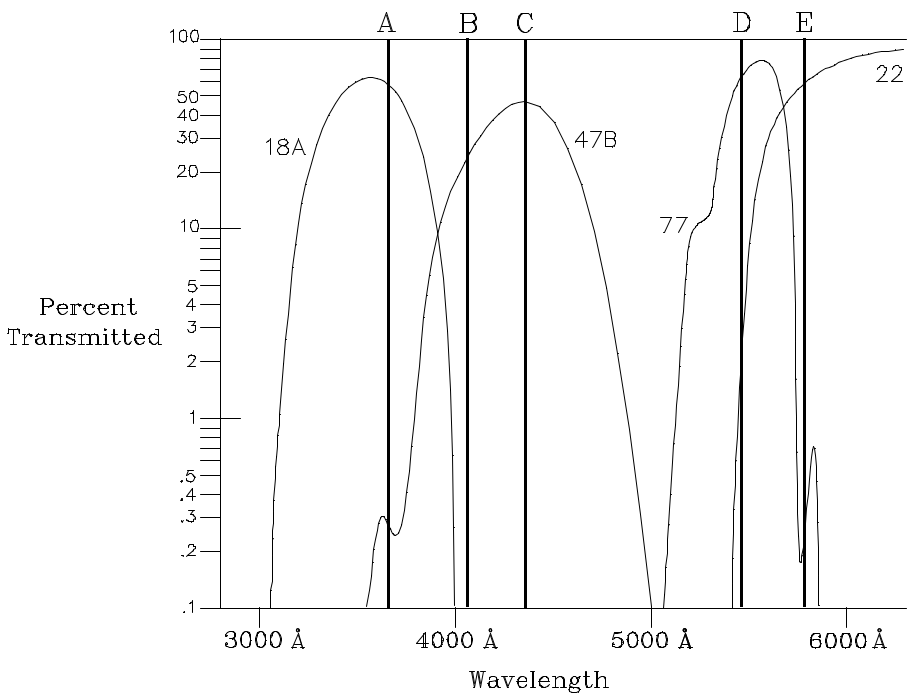
\includegraphics[width=0.8\textwidth]{./Exp8/pic/image7.png}
\caption{Creation and Detection of Polarized Light}
\label{fig:polarized}
\end{figure}

\subsection{Double Slit}
In this part of the experiment we use a laser instead of incandescent light source. Laser light shines onto a double slit, which produces an interference pattern of bright and dark lines on the wall or a piece of paper beyond the double slit. \myskip

We know that the angle, $\theta_{m}$, at which the $m^{\mathrm{th}}$ order bright spot appears is given by
\begin{equation}
 d\sin\theta_{m}=m\lambda
\end{equation}

For small $\theta_{m}$ (in radians), the approximation $\sin\theta \approx \tan\theta \approx \theta$ is valid\footnote{See for yourself by punching $\sin 0.1$ and $\tan 0.1$ into your calculator (using radiant measure)!}. So on a screen far away from the double slit, we observe maxima located close to the optical axis (where the $0^{\mathrm{th}}$ order maximum hits the screen) approximately given by
\begin{equation}
\sin\theta_{m}\approx\tan\theta_{m}=\frac{x_{m}}{L}
\end{equation}
where $x_m$ is the distance between the $m^{\mathrm{th}}$ order maximum and the $0^{\mathrm{th}}$ order maximum, and $L$ is the distance between the double slit and the screen. We then find
\begin{equation}
\frac{x_{m}}{L}=m\frac{\lambda}{d}
\end{equation}
or for adjacent maxima
\begin{equation}
 \frac{\Delta x}{L}=\frac{\lambda}{d}
\end{equation}
with $\Delta x$ equal to the distance between the maxima. Since $\Delta x$ and $L$ are easy to measure, we can straightforwardly determine $d$ (or $\lambda$ ) given $\lambda$ (or $d$).

\section{Specifics of the Experiment}
\underline{SAFETY NOTE:}

\emph{Although the laser is of low intensity for most situations, it can be dangerous in certain circumstances unless used carefully. In particular, \textbf{do not} use the laser in such a way that it can shine into any person's eye (The warning label on the laser states ``Do not stare into Beam!''). When you are not actually using the laser, turn it off or close the beam shutter at the front of the laser.}
\begin{figure}[h]
\centering
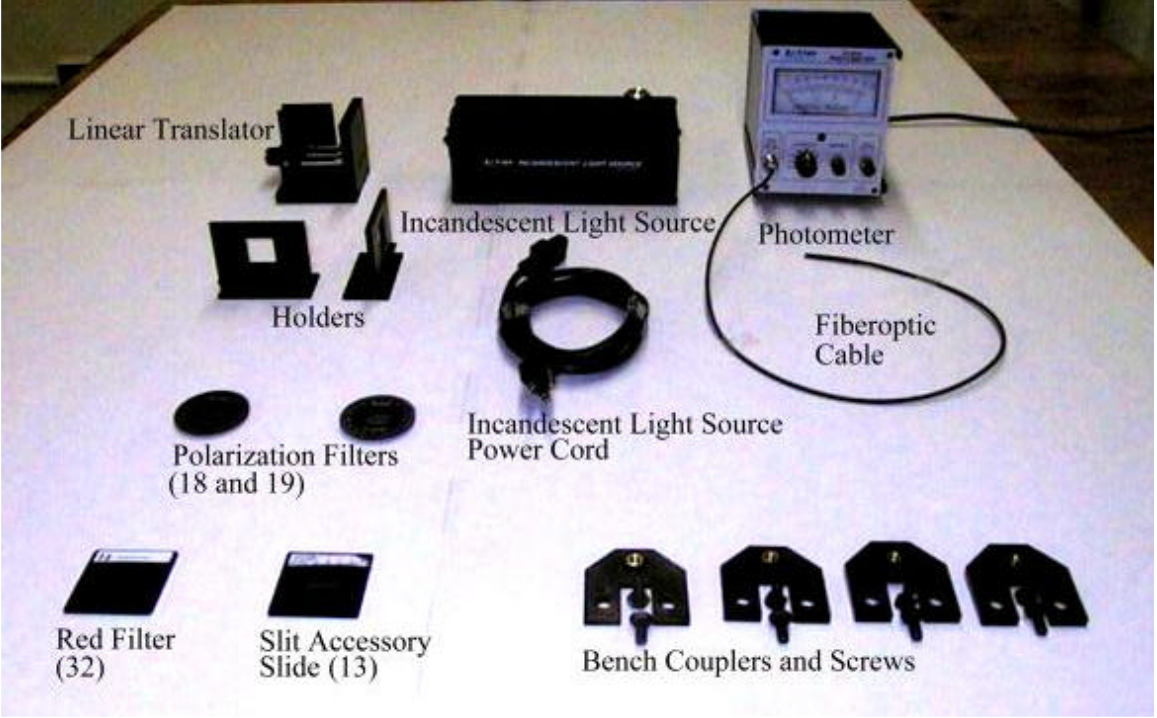
\includegraphics[width=0.8\textwidth]{./Exp8/pic/image8.png}
\caption{Equipment Components}
\label{fig:setup}
\end{figure}

\section{Equipment}
\indent\indent\underline{Linear Translator:}
A holder for the fiberoptic cable that can be moved transversely in small increments, allowing a positioning with better than $0.1\,\mathrm{mm}$ precision. \myskip

\underline{Fiberoptic Cable:}
Cable made from glass, quartz, plastic or a similar material, which carries light waves. The cable uses total internal reflection at the walls to provide very high efficiency (or low losses) between the cable ends.\myskip

\underline{Photometer:}
Device to measure the total power contained in light impinging on it. It uses the photoelectric effect to convert the photons to electrons and various electron amplification techniques to produce a measurable electric current.

\subsection{Polarization}
\begin{enumerate}
\item Make sure only the dim incandescent ceiling lights in the room are on.

\item The linear translator should be placed at the far end of the track opposite the laser. Make sure that the linear translator is in the middle position (at $2.5\,\mathrm{cm}$).

\item Place the fiber-optic cable in the hole of the linear translator.

\item Place the incandescent light source about $10$-$20\,\mathrm{cm}$ from the linear translator such that the light shines towards the linear translator.

\item Place the polarizers (numbers 18 and 19) in the holders.

\item Rotate each polarizer such that the white mark on the holder aligns with the $0^{\circ}$ angle reading on the polarizer.

\item Place the two polarizers between the incandescent light source and the linear translator.

\item Set the photometer to the lowest sensitivity (the 1000 setting) and use the zero adjust knob to make sure that the pointer is at the 0 position when the incandescent light source is turned off.

\item Turn the incandescent light source back on and adjust the sensitivity of the photometer such that the needle is at the highest position without being at the maximum reading. The value of the sensitivity corresponds to the maximum value on the analog scale.

\item Record this measurement as the intensity for $0^{\circ}$ difference between the two polarizing axes.

\item Begin by rotating one of the polarizers by 10 degrees and measure the intensity. Continue measuring the intensity for angles between $0^{\circ}$ and $90^{\circ}$ in increments of 10 degrees. If the readings become too small you may have to switch the photometer to a setting with a higher sensitivity. Make sure you are always keeping one polarizer aligned at $0^{\circ}$.

\item Plot the relative intensity ($I$ divided by $I_0$, the intensity at $0^{\circ}$) vs. the $\cos^2\theta$ where $\theta$ is the angle between the axes of your polarizers. Be sure to include error bars on both axes and a line of best-fit. You can determine the error in $I/I_0$ by examining the precision of the photometer. You can determine the error in $\cos^2\theta$ using the following equation:
\begin{equation}
 \sigma_{\cos^2\theta} = 2\cos(\theta)\sin(\theta)\sigma_{\theta}
\end{equation}

\item Determine the slope and intercept o your plot with error found using LINEST. What values do you expect for the slope and intercept? Do your measured values agree within error?

\item What reading do you obtain when the polarizers are at an angle of $90^{\circ}$ relative to each other? (This is called the ``noise'' of your measuring device.) What reading would you expect if there was no noise?

\item If you had a lot of background light, how could you reduce the influence it would have on your results (by changing the setting or by changing your data analysis)?

\item If you had aligned the $90^{\circ}$ mark instead of the $0^{\circ}$ mark of both polarizers with the white mark on the holder would your results have been any different? What relative intensity would you expect if the angle between the two polarizers was $180^{\circ}$? $270^{\circ}$?

\item What are the main sources of error? Which do you think contributes most?
\end{enumerate}

\subsection{Double Slit}
\begin{enumerate}
\item Before you start this section, be sure you have read the laser safety note above.

\item Your TA will demonstrate the interference pattern by projecting it on the wall. Note down your observations!

\item Remove the incandescent light source, the polarizers, and the holders from the track, and the fiberoptic cable from the linear translator.

\item The laser should already be mounted on the laser holder at the far end of the track. Rotate the dial on the linear translator so that it is in the middle position.

\item Turn on the laser. It should propagate through the center of the hole in the linear translator, producing a bright red dot on the wall. If the laser is not properly aligned, alter the position of the laser by adjusting \emph{only the back legs} on the laser holder. Make sure you avoid lifting the laser and shining it in your classmates' eyes.

\item Place the red filter (number 32) onto the linear translator. Carefully slide the fiberoptic cable back into the hole in the linear translator so that the front of the cable sits right against the red filter.

\item Place the slide with the slits (number 13) in a holder and place the holder right in front of the laser.

\item Adjust the slide position in the holder so that the laser propagates through slit pattern A.

\item Note the interference pattern on the front of the linear translator.

\item Adjust the photometer sensitivity to an appropriate setting. Try turning the knob on the linear translator. This should cause the intensity reading on the photometer to change. You should notice the intensity has various maxima.

\item Move the linear translator as far as possible, starting from the 0 position of the linear translator. Record the position and intensity for each maximum. As you turn the knob on the linear translator, take care not to shift the position of the linear translator on the bench.

\item Where do you see the $0^{\mathrm{th}}$ order maximum (the tallest peak from Figure \ref{fig:intensity})? Why might it be located somewhere other than the middle position of the linear translator?

\item Measure and record the distance $L$ from the position of the slits to the tip of the fiberoptic cable.

\item With Microsoft Excel, plot the position of the maxima $x_m$ vs. the order $m$. Only include error bars for the position. Determine the slope of your line of best-fit and use it to calculate the wavelength of the laser light with error using LINEST. Note that the slit separation for slit A is 0.250 mm.

\item With Microsoft Excel, pot the relative intensity, $I/I_0$ vs. $x_m$. Explain the shape of your graph.

\item What is the purpose of using the red filter?

\item Discuss the main sources of error in this experiment.
\end{enumerate}

\section{Applications}
Some chemical molecules have a property called chirality. This means that the mirror image of the molecule is not identical to the original. For example, no matter how good you might be at 3D puzzles, you cannot arrange images of the molecule and of its mirror image to superimpose precisely. A famous example is the DNA double helix, a highly complex molecule, which carries all genetic information. The molecule always twists in one direction, while its mirror image always twists in the opposite direction. Many such chiral molecules are optically active, and rotate the polarization-axis of transmitted or reflected polarized light\footnote{For instance, the glucose dextrose turns the polarization axis to the right: ``dexeter'' is Latin for ``right''.}. If you shine polarized light into such a sample, you will see that the light leaving the sample has its polarization axis rotated a few degrees clockwise or counterclockwise, depending on the substance.\myskip

This effect can be used to determine the concentration of chiral molecules in a solution. For example, you can determine the glucose concentration in a blood specimen in a non-chemical way. The calculation of the concentration is particularly simple, since the change in angle of the polarization axis depends only on the concentration of the chiral substance in the solution, the distance the light travels through the sample, and a constant specific for the substance. Calculating the glucose concentration, therefore, requires only a measurement of the rotation in polarization vector and known constants -- a simple task for a rudimentary computer.

\newpage
\section{Lab Preparation Examples}
\underline{Polarization:}
\begin{enumerate}
\item You look at the sky through a polarizer and as you turn the polarizer you see that the sky appears darker or lighter, depending on the position of the polarizer. What does this observation tell you?

\item You look at a light source through a polarizer. As you turn the polarizer you see no change in intensity. Is the light emitted by this source polarized?

\item Unpolarized light passes through two polarizers whose polarization axes are aligned. You note down the observed intensity as $I_{0}$. Now you turn the polarization axis of one of the polarizers by $60^{\circ}$. What intensity do you observe now?

\item Now you add, after the second polarizer, a third polarizer. The third has a polarization axis of $30^{\circ}$ relative to the second polarizer. What intensity do you observe now?

\item Does the result depend on which of the two polarizers you rotate in question 3?

\item Would your answer to question 5 change if the light source produced polarized light? Explain!

\item You have two polarizers with an angle of $90^{\circ}$ between their polarization axes. Adding a third polarizer between these two polarizers will typically produce light after the final polarizer. At what angle (relative to the first polarizer's axis) would you observe the maximum intensity after the third polarizer?
\end{enumerate}

\underline{The Double-Slit:}

While performing a double slit experiment, with $L = 1.00\pm 0.01\,\mathrm{m}$, $d = 0.5\pm 0.1\, \mathrm{mm}$, you obtain the following locations for maxima:
\begin{table}[h]
 \centering
 \begin{tabular}{|c|c|c|c|c|c|c|c|c|c|}
  \hline
  order&-4&-3&-2&-1&0&1&2&3&4\\
  \hline
  Position (mm)&-4.1&-3.2&-2.0&-0.9&0.0&1.3&2.1&3.2&3.9\\
  \hline
 \end{tabular}
\end{table}
\begin{enumerate}\setcounter{enumi}{7}
\item Calculate x for all of the consecutive maxima and use the 2/3 estimate to determine the uncertainty of x. Now determine the wavelength of the light (including uncertainty).
\item Using the data above, determine x from a plot of position vs. order. Given the wavelength as $\lambda = 600\,\mathrm{nm}$ and $L = 1.00\pm 0.01\,\mathrm{m}$, what is the spacing between the two slits?
\end{enumerate}

\section{Appendix for Experts: How a Laser works (Not required!)}
Quantum mechanics tells us that light is produced when electrons in an atom make a transition from a higher to a lower state, or energy level. Whenever an electron makes a
transition between states, the difference in energy is emitted (or absorbed) as a discrete energy package called a photon\footnote{See the experiment on the Photoelectric Effect.}, which carries (with other photons) the electromagnetic wave. The transition from a higher to a lower state can happen in two different ways. First, it can happen randomly, i.e. the electron just falls down spontaneously. This is what happens when a candle produces light. Electrons that make such random transitions result in emitted photons which are incoherent, or out of phase with one another. \myskip
\begin{figure}[h]
\centering
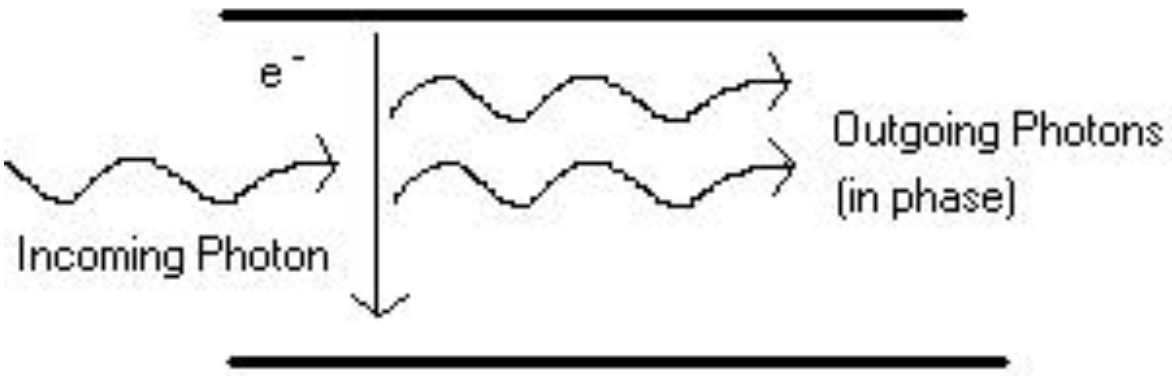
\includegraphics[width=0.5\textwidth]{./Exp8/pic/image9.png}
\caption{Process of Stimulated Emission}
\label{fig:stimulatedemission}
\end{figure}

The second way this process can happen is called stimulated emission. If you already have a field of photons that are in phase and have the same frequency, and that frequency corresponds exactly to the transition energy, the emission is no longer random. When an electron falls to the lower energy level, a photon is emitted precisely in phase with the already existing photons, as shown in Figure {\ref{fig:stimulatedemission}}.\footnote{Photons are of a particle type called bosons. Such particles are highly ``social'' and like to be in exactly the same energy state and the same phase with their friends. This contrasts with another particle type, called fermions, which hate being in the same state as their associates (Pauli Exclusion Principle). Electrons are fermions, and this antisocial property accounts for the unique state of each electron in an atom. If electrons were bosons, all electrons in an atom would be in the ground state and we would not have chemistry!} In our analogy of soldiers marching on parade, new entrants to the parade are required to start walking in step with the others (or they would miss out on the parade).\myskip
\begin{figure}[h]
\centering
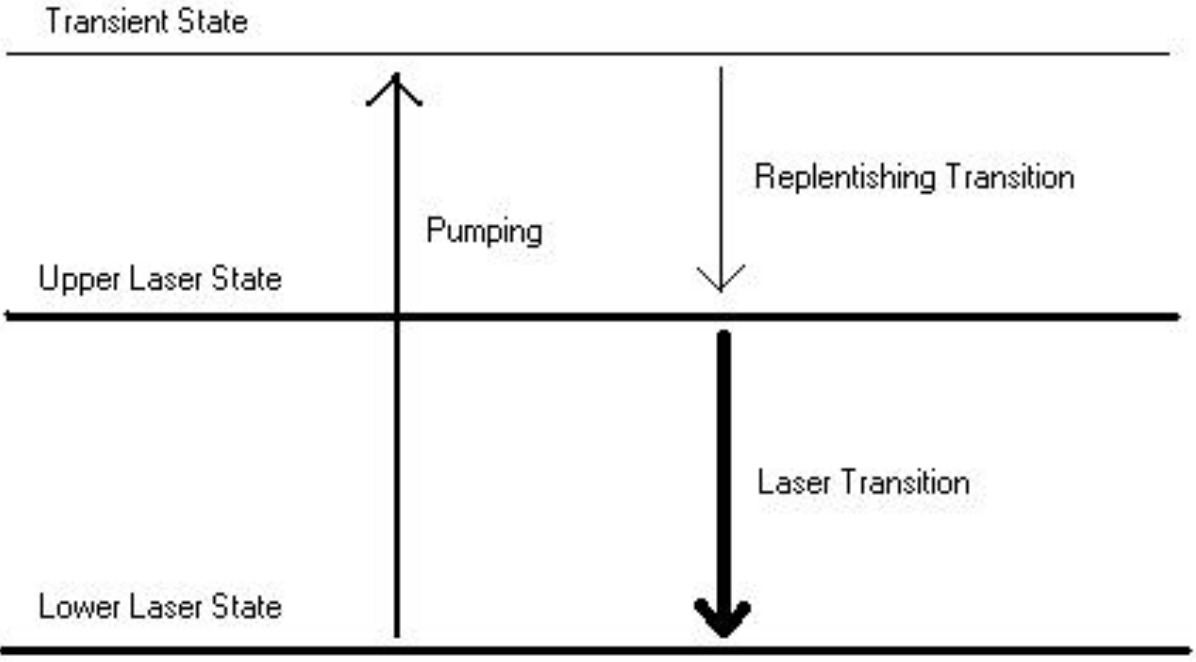
\includegraphics[width=0.5\textwidth]{./Exp8/pic/image10.png}
\caption{The basic three - level scheme for laser operation.}
\label{fig:transition}
\end{figure}

For stimulated emission to work, the upper atomic state must be full of electrons and the lower one must be almost empty. This is called an inversion, since atoms (at ordinary temperatures) tend to be in their lowest energy state. The inversion is actually achieved by pumping the electrons from the lower state into a third transient state, with an energy even higher than the second laser state, so that the electrons fall down to replenish the upper laser state. So real lasers use at least three energy levels; efficient lasers usually use even more\footnote{Semiconductor lasers (or laser diodes) work somewhat differently, but the underlying concepts of stimulated emission and inversion are the same.}.\myskip

Finally, the setup is placed in a cavity with a mirror at one end and a semi-transparent\footnote{These semi-transparent mirrors are still highly reflective. They reflect about 99$\%$ of incident light to keep most of the light inside the cavity.} mirror at the other end. This increases the efficiency of the laser by maintaining a high density of laser light within the cavity. The little leakage emitted from the semitransparent mirror is actually what we use as the laser beam.
